
\documentclass[10pt]{article}
\usepackage[a4paper, tmargin=0.75in, lmargin=0.80in, rmargin=0.80in, bmargin=1in]{geometry}
\usepackage{hyperref}
\usepackage{dsfont}
\usepackage{amsfonts}
\usepackage{ragged2e}
\usepackage{mathtools}
\usepackage{enumitem}   
\usepackage{MnSymbol}%
\usepackage{wasysym}%
\usepackage{relsize}%
\usepackage{xcolor}

\usepackage{amsmath}
\usepackage{upgreek}
\usepackage{mathrsfs}
\usepackage{blindtext}
\usepackage{listings}
\usepackage{xcolor}


%New colors defined below
\definecolor{codegreen}{rgb}{0,0.6,0}
\definecolor{codegray}{rgb}{0.5,0.5,0.5}
\definecolor{codepurple}{rgb}{0.58,0,0.82}
\definecolor{backcolour}{rgb}{0.95,0.95,0.92}

\lstset{
    literate={ĉ}{{\^c}}1
        {Ĉ}{{\^C}}1
}

%Code listing style named "mystyle"
\lstdefinestyle{mystyle}{
  backgroundcolor=\color{backcolour}, commentstyle=\color{codegreen},
  keywordstyle=\color{magenta},
  numberstyle=\tiny\color{codegray},
  stringstyle=\color{codepurple},
  basicstyle=\ttfamily\footnotesize,
  breakatwhitespace=false,         
  breaklines=true,                 
  captionpos=b,                    
  keepspaces=true,                 
  numbers=left,                    
  numbersep=5pt,                  
  showspaces=false,                
  showstringspaces=false,
  showtabs=false,                  
  tabsize=2
}

\lstset{style=mystyle}


\usepackage{natbib}
\usepackage{graphicx}
\pagestyle{empty}
\renewcommand\thesubsection{\Alph{subsection}}
\DeclareMathOperator*{\limop}{\lim}




%%%%%%%%%%%%%%%%%%%%%%%%%%%%%%%%%%%%%%%%%%%%%%%%%%
%%%%%%%%%%%%%%%%%%%%%%%%%%%%%%%%%%%%%%%%%%%%%%%%%%
%%%%%%%%%%%%%%%%%%%%%%%%%%%%%%%%%%%%%%%%%%%%%%%%%%
%%%%%%%%%%%%%%%%%%%%%%%%%%%%%%%%%%%%%%%%%%%%%%%%%%
% ENTER SOME IMPORTANT INFORMATION
%%%%%%%%%%%%%%%%%%%%%%%%%%%%%%%%%%%%%%%%%%%%%%%%%%
%%%%%%%%%%%%%%%%%%%%%%%%%%%%%%%%%%%%%%%%%%%%%%%%%%
%%%%%%%%%%%%%%%%%%%%%%%%%%%%%%%%%%%%%%%%%%%%%%%%%%
%%%%%%%%%%%%%%%%%%%%%%%%%%%%%%%%%%%%%%%%%%%%%%%%%%
\newcommand{\studentname}{Luis Alejandro Rubiano}
\newcommand{\studentnumber}{202013482}
\newcommand{\researchcentre}{la.rubiano@uniandes.edu.co}
\newcommand{\projecttitle}{Convex Optimization}
\newcommand{\supervisor}{Mauricio Junca}
\newcommand{\xRightarroww}[2][]{\ext@arrow 0359\Rightarrowfill@{#1}{#2}}

\newcommand\setItemnumber[1]{\setcounter{enum\romannumeral\@enumdepth}{\numexpr#1-1\relax}}

\newcommand\restr[2]{{% we make the whole thing an ordinary symbol
  \left.\kern-\nulldelimiterspace % automatically resize the bar with \right
  #1 % the function
  \littletaller % pretend it's a little taller at normal size
  \right|_{#2} % this is the delimiter
  }}

\newcommand{\littletaller}{\mathchoice{\vphantom{\big|}}{}{}{}}


%%%%%%%%%%%%%%%%%%%%%%%%%%%%%%%%%%%%%%%%%%%%%%%%%%
%%%%%%%%%%%%%%%%%%%%%%%%%%%%%%%%%%%%%%%%%%%%%%%%%%
%%%%%%%%%%%%%%%%%%%%%%%%%%%%%%%%%%%%%%%%%%%%%%%%%%
%%%%%%%%%%%%%%%%%%%%%%%%%%%%%%%%%%%%%%%%%%%%%%%%%%
%%%%%%%%%%%%%%%%%%%%%%%%%%%%%%%%%%%%%%%%%%%%%%%%%%
%%%%%%%%%%%%%%%%%%%%%%%%%%%%%%%%%%%%%%%%%%%%%%%%%%

\begin{document}

\begin{center}
{\Huge{Homework 2, Convex Optimization}} \\
\vspace{2mm}
{\Large{Departamento de Matemáticas, Universidad de los Andes}} \\
\vspace{1mm}
{\Large{Colombia}}
\end{center}

\vspace{5mm}
\hrule
\vspace{1mm}
\hrule

\vspace{3mm}
\begin{tabular}{ll} 
Student's name:           	        & {\studentname}   \\ 
Student's code: 	        & {\studentnumber} \\ 
Email address: 	        & {\researchcentre}  \\ 
Class: 	& {\projecttitle}  \\ 
Instructor: 	    & {\supervisor}  \\ 
\end{tabular}

\vspace{3mm}
\hrule
\vspace{1mm}
\hrule

\hfill \break %SPACE

\section{Find the minimum over $\mathbb{R}_{++}^2$ of the function $f(x,y) = \frac{1}{xy} + x + y$.}



\paragraph{Solution:}


The function $\cfrac{1}{xy}$ has hessian matrix given by $
\begin{pmatrix}
\cfrac{2}{x^3y} & \cfrac{1}{x^2y^2} \\
\cfrac{1}{x^2y^2} & \cfrac{2}{xy^3} 
\end{pmatrix}
$. 

Then let $a,b \in \mathbb{R}$, let $v=\cfrac{a}{x^{3/2} y^{1/2}}$ and $w=\cfrac{b}{x^{1/2} y^{3/2}}$, then for $x,y \geq 0$ we have that 

\begin{align*}
    \begin{pmatrix}
        a & b \\
    \end{pmatrix} \begin{pmatrix}
        \cfrac{2}{x^3y} & \cfrac{1}{x^2y^2} \\
        \cfrac{1}{x^2y^2} & \cfrac{2}{xy^3} 
        \end{pmatrix}
        \begin{pmatrix}
        a \\
        b
    \end{pmatrix} &= 2 \left( \cfrac{a^2}{x^3y} + \cfrac{b^2}{xy^3} + \cfrac{ab}{x^2 y^2} \right)\\
    &= 2 \left( v^2 + w^2 + vw \right)\\
\end{align*}

Note that this last expression can only be negative if either $v$ or $w$ is negative, but this is not possible since 
w.l.o.g. assume $v<0<w$ then 
\begin{itemize}
    \item Case 1: if $-v \leq w$ then $-vw \leq w^2$ or $0 \leq w^2 + vw$.
    \item Case 2: if $w<-v$ then $-vw < v^2$ or $0 < v^2 + vw$.
\end{itemize}

Therefore, $2 \left( \cfrac{a^2}{x^3y} + \cfrac{b^2}{xy^3} + \cfrac{ab}{x^2 y^2} \right) \geq 0$ for all $a,b \in \mathbb{R}$ and $x,y \geq 0$ 
and the hessian matrix is positive semidefinite. 

Then the function $f(x,y) = \cfrac{1}{xy} + x + y$ is convex over $\mathbb{R}_{++}^2$ since its the sum of convex functions.

Therefore the minimum of $f(x,y)$ over $\mathbb{R}_{++}^2$ is the point where the gradient of $f(x,y)$ is zero. 

The gradient of $f(x,y)$ is given by $\nabla f(x,y) = \begin{pmatrix}
-\cfrac{1}{x^2 y} + 1 \\
-\cfrac{1}{xy^2} + 1
\end{pmatrix}$, setting it equal to zero we get that $x=y=1$ is the only point where the gradient is zero, and since the hessian is positive semidefinite, then $x=y=1$ is the minimum of $f(x,y)$ over $\mathbb{R}_{++}^2$.


\hfill \break %SPACE

\section{Consider the function $f(x,y) = x^2 - \alpha xy^2 + 2 y^4$. Show that for all 
parameter values except two, the origin $(0,0)$ is the only critical point of $f$. Ex. 2.9 Foundations of Optimization, Güller}


\begin{enumerate}[label=(\alph*)]
    \item Find the exceptional $\alpha$'s and show that $f$ has infinitely many critical points for these $\alpha$ values. Determine the nature of these critical points.
\end{enumerate}

\paragraph{Solution:}

Note that $f$ is a polynomial in two variables, thus when calculating the directional derivative of $f$ at 
a point $(x_0,y_0)$ in the direction of a vector $(d_1,d_2)$ we have that
$f(x_0 + td_1, y_0 + td_2) - f(x_0,y_0)$ will also be a polynomial in $t$, 
thus when dividing by $t$ and taking the limit as $t$ goes to zero, the higher 
order terms will vanish and we will be left with only the linear terms, which implies 
that the directional derivative of $f$ at $(x_0,y_0)$ in the direction of $(d_1,d_2)$, exists and is a linear.\\

Then the gradient of $f$ is given by $\nabla f(x,y) = \begin{pmatrix}
2x - \alpha y^2 \\
-2\alpha xy + 8y^3\\
\end{pmatrix}$, setting it equal to zero we get:

\begin{align}
    2x - \alpha y^2 &= 0\\
    -2\alpha xy + 8y^3 &= 0
\end{align}

$$\Rightarrow x = (\alpha y^2)/2$$

Replacing this into the second equation we get that 

\begin{align*}
    -2\alpha y(\alpha y^2)/2 + 8y^3 &= 0\\
    -\alpha^2 y^3 + 8y^3 &= 0\\
    (8-\alpha^2)y^3 &= 0
\end{align*}

Then, the only way for this equation to hold is if $y=0$ or $8-\alpha^2=0$, the first case implies that $x=0$ and the second case implies that $\alpha = \pm 2\sqrt{2}$.\\

When $\alpha = 2\sqrt{2}$, setting the gradient of $f$ equal to zero we get:

\setcounter{equation}{0}

\begin{align}
    2x - 2\sqrt{2} y^2 &= 0\\
    -4\sqrt{2} xy + 8y^3 &= 0
\end{align}

Setting the two equations, equal to each other, we get that the set of solutions is 
given by the parabola $x = \sqrt{2} y^2$, which has infinitely many points.\\

In an analogous way, when $\alpha = -2\sqrt{2}$, setting the gradient of $f$ equal to zero we get
that the set of solutions is given by the parabola $x = -\sqrt{2} y^2$, which has infinitely many points.\\

To see the nature of the critical points, we can see that by the same argument as before, each entry of $\nabla f(x,y)$ is a polynomial in $x$ and $y$, thus the hessian of $f$ is well defined.\\

Then, the hessian of $f$, with $\alpha = 2\sqrt{2}$ is given by

$$H_f(x,y) = \begin{pmatrix}
2 & -2\sqrt{2}y \\
-2\sqrt{2}y & -8\sqrt{2}x + 24y^2
\end{pmatrix}$$

Evaluating at the parabola, using the substitution $x := \sqrt{2} y^2$ we get that

$$H_f(\sqrt{2} y^2, y) = \begin{pmatrix}
2 & -2\sqrt{2}y \\
-2\sqrt{2}y & 32y^2\\
\end{pmatrix}$$

This matrix has eigenvalues $1 + 16y^2 - \sqrt{1+256y^4}$ and $1 + 16y^2 + \sqrt{1+256y^4}$, which are both positive for all $y \neq 0$, thus the hessian is positive definite 
except at the origin, where it is positive semidefinite. When $y \neq 0$  the critical points are strict local minimizers. The case for $\alpha = -2\sqrt{2}$ is analogous by symmetry.\\ 




\begin{enumerate}[label=(\alph*)]
    \setcounter{enumi}{1}
    \item Consider the values of $\alpha$’s for which the origin is the only critical point. For each $\alpha$, determine the nature of the critical point. Show that in some cases, the origin is a local minimum, but in other cases, it is a saddle point.
\end{enumerate}

\paragraph{Solution:}

We claim the following: When $- 2 \sqrt{2} < \alpha < 2 \sqrt{2}$, the origin is a global minimum. To see this, we can complete the square
and see $f(x,y) = x^2 - \alpha xy^2 + 2 y^4 = x^2 + y^2(2y^2-\alpha x) = \left(x-\cfrac{\alpha y^2}{2}\right)^2 + \left(2 - \cfrac{\alpha^2}{4}\right)y^4$.\\

The first term is squared, thus always greater or equal to zero, and the second term is positive when $- 2 \sqrt{2} < \alpha < 2 \sqrt{2}$, thus since $f(0,0) = 0$, and $f(x,y) > 0$ for all $(x,y) \neq (0,0)$, then the origin is a global minimum.\\

When $\alpha \in \mathbb{R} \setminus [- 2 \sqrt{2}, 2 \sqrt{2}]$, the origin is a saddle point. W.L.O.G assume $\alpha > 2 \sqrt{2}$, the other case is completely analogous. To see this, in the previous point
we already showed the origin it is a critical point, we can now take $\varepsilon>0$. Then, $f(\cfrac{\alpha \varepsilon^2}{2}, \varepsilon) = - \cfrac{\alpha^2 \varepsilon^4}{4} + 2 \varepsilon^4 = y^4(2 - \cfrac{\alpha^2}{4}) < 0$, but moving along the $x$ axis, we have that $f(\varepsilon,0) = \varepsilon^2 > 0$, thus by definition the origin is a saddle point.\\






\begin{enumerate}[label=(\alph*)]
    \setcounter{enumi}{2}
    \item Show that even when the origin is a saddle point, $(0,0)$ is a local strict minimizer of $f$ on every line passing through the origin. In fact, show that, except for one line, the function $g(t):=f(td)$ satisfies $g'(0) =0$ and $g''(0)>0$.
\end{enumerate}

\paragraph{Solution:}

Note that when substituting $g(t) := f(td) = (td_1)^2 - \alpha (td_1) (td_2)^2 + 2 (t d_2)^4$, 

We get that $g'(t) = 2t d_1^2 - 3 \alpha d_1 d_2^2 t^2 + 8 d_2^4 t^3$ and 
$g''(t) = 2 d_1^2 - 6 \alpha d_1 d_2^2 t + 24 d_2^4 t^2$.\\

Then, $g'(0) = 0$ and $g''(0) = 2 d_1^2 > 0$, except for the line $d_1 = 0$, where $g''(0) = 0$.\\



\hfill \break %SPACE

\section{Program the steepest descent and Newton algorithms using the backtracking line search, Algorithm 3.1.
Use them to minimize the Rosenbrock function (2.22). Set the initial step length
$\alpha_0= 1$, and print the step length used by each method at each iteration. First try the initial point
$x_0 = (1.2, 1.2)^T$ and then the more difficult starting point $x_0 = (-1.2, 1)^T$. Ex. 3.1. Numerical Optimization, Nocedal \& Wright}


\paragraph{Solution:}

Python3 code to solve this problem is given by:

\begin{lstlisting}[language=Python]
    import sympy as sp
    import matplotlib.pyplot as plt
    import os
    
    x_1, x_2 = sp.symbols('x_1 x_2')
    
    f = 100 * (x_2 - x_1**2)**2 + (1 - x_1)**2
    
    
    def steepest_descent(x_k, gradient, hessian):
        # Returns the gradient at x_k
        return - gradient.subs({x_1: x_k[0], x_2: x_k[1]})
    
    
    def newton(x_k, gradient, hessian):
        # Returns - H^-1 evaluted at x_k times the gradient at x_k
        return - hessian.subs({x_1: x_k[0], x_2: x_k[1]}).inv() * \
            gradient.subs({x_1: x_k[0], x_2: x_k[1]})
    
    
    def graph(x, y, title, x_label, y_label, filename):
        fig = plt.figure()
        plt.plot(x, y)
        plt.title(title)
        plt.xlabel(x_label)
        plt.gca().xaxis.set_major_locator(plt.MaxNLocator(integer=True))
        plt.ylabel(y_label)
        filename = "Tarea2" + os.sep + "images" + os.sep + filename + ".png"
        fig.savefig(filename, dpi=fig.dpi)
        plt.clf()
    
    
    def minimize(f, x_0, method, a_0):
        rho = 0.5
        c = 0.5
        iterations = 0
        max_iterations = 20
    
        gradient = sp.Matrix([f.diff(x_1), f.diff(x_2)])
        hessian = sp.hessian(f, (x_1, x_2))
    
        if method == 'steepest_descent':
            p = steepest_descent
        elif method == 'newton':
            p = newton
    
        X = [x_0]
        F = [f.subs({x_1: x_0[0], x_2: x_0[1]})]
        A = [a_0]
        P = []
    
        P.append(p(X[-1], gradient, hessian))
    
        while iterations < max_iterations:
            while f.subs({x_1: X[-1][0] + A[-1] * P[-1][0],
                          x_2: X[-1][1] + A[-1] * P[-1][1]}) > f.subs({x_1: X[-1][0],
                                                                       x_2: X[-1][1]}) + c * A[-1] * gradient.subs({x_1: X[-1][0],
                                                                                                                    x_2: X[-1][1]}).dot(P[-1]):
                A[-1] = rho * A[-1]
    
            X.append(X[-1] + A[-1] * P[-1])
            F.append(f.subs({x_1: X[-1][0], x_2: X[-1][1]}))
            P.append(p(X[-1], gradient, hessian))
            A.append(a_0)
    
            iterations += 1
    
        return X, F, A[:-1], P
    
    
    X, F, A, P = minimize(f, x_0=sp.Matrix(
        [1.2, 1.2]), method='steepest_descent', a_0=1)
    
    graph([i for i in range(len(A))],
          A,
          r"Step size, using Steepest Descent, $x_0 = [1.2, 1.2]$",
          "Iteration",
          r"$\alpha$",
          "steepest_descent_step_size_a")
    graph([i for i in range(len(F))],
          F,
          r"$f(x)$, using Steepest Descent, $x_0 = [1.2, 1.2]$",
          "Iteration",
          r"$f(x)$",
          "steepest_descent_fx_a")
    
    X, F, A, P = minimize(f, x_0=sp.Matrix([1.2, 1.2]), method='newton', a_0=1)
    
    graph([i for i in range(len(A))],
          A,
          r"Step size, using Newton, $x_0 = [1.2, 1.2]$",
          "Iteration",
          r"$\alpha$",
          "newton_step_size_a")
    graph([i for i in range(len(F))],
          F,
          r"$f(x)$, using Newton, $x_0 = [1.2, 1.2]$",
          "Iteration",
          r"$f(x)$",
          "newton_fx_a")
    
    X, F, A, P = minimize(f, x_0=sp.Matrix(
        [-1.2, 1]), method='steepest_descent', a_0=1)
    
    graph([i for i in range(len(A))],
          A,
          r"Step size, using Steepest Descent, $x_0 = [-1.2, 1]$",
          "Iteration",
          r"$\alpha$",
          "steepest_descent_step_size_b")
    graph([i for i in range(len(F))],
          F,
          r"$f(x)$, using Steepest Descent, $x_0 = [-1.2, 1]$",
          "Iteration",
          r"$f(x)$",
          "steepest_descent_fx_b")
    
    X, F, A, P = minimize(f, x_0=sp.Matrix([-1.2, 1]), method='newton', a_0=1)
    
    graph([i for i in range(len(A))],
          A,
          r"Step size, using Newton, $x_0 = [-1.2, 1]$",
          "Iteration",
          r"$\alpha$",
          "newton_step_size_b")
    graph([i for i in range(len(F))],
          F,
          r"$f(x)$, using Newton, $x_0 = [-1.2, 1]$",
          "Iteration",
          r"$f(x)$",
          "newton_fx_b")
\end{lstlisting}

\begin{figure}[!tbp]
    \centering
    \begin{minipage}[b]{0.4\textwidth}
        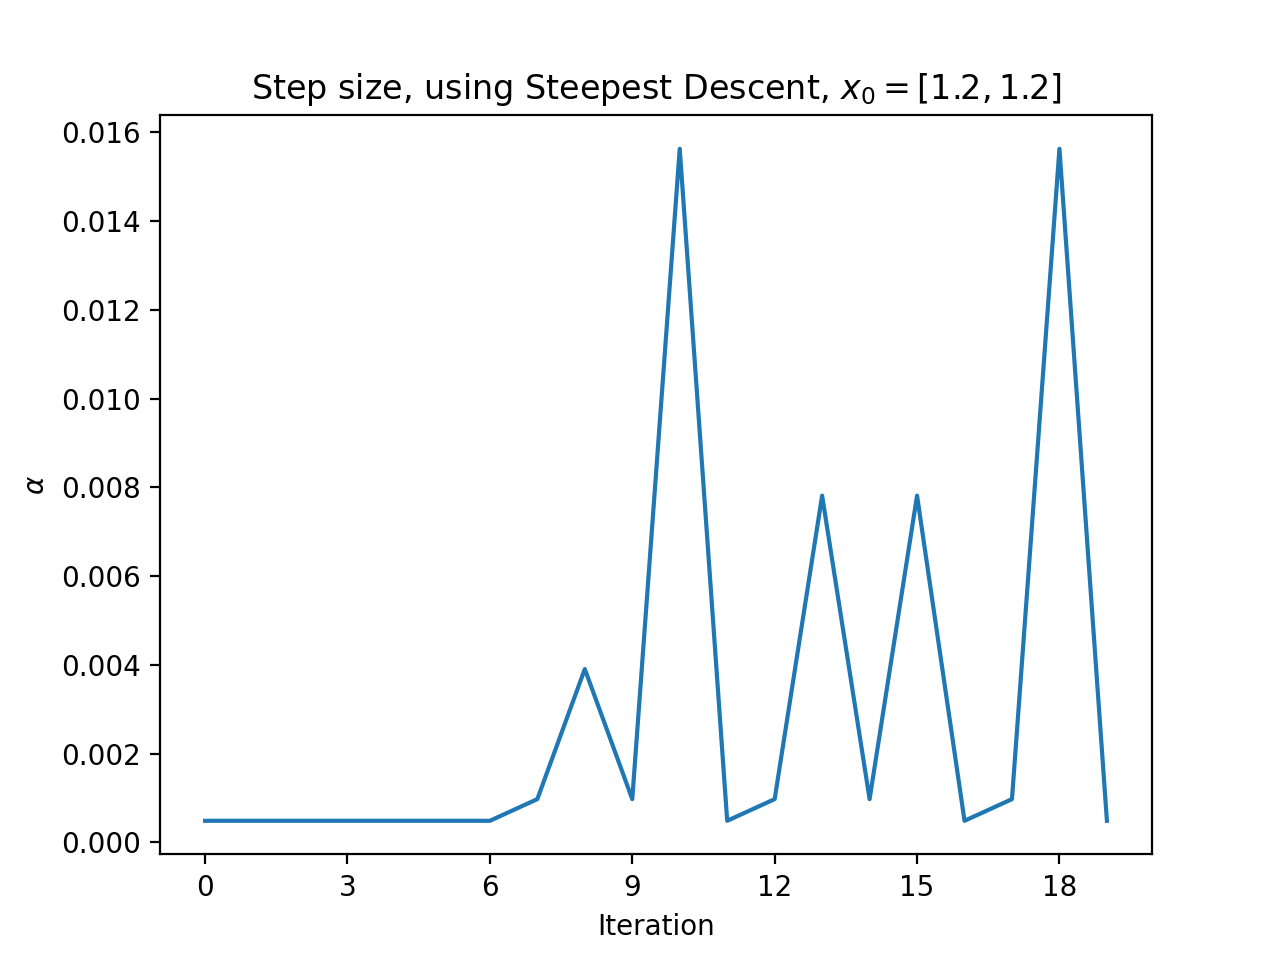
\includegraphics[width=\textwidth]{images/steepest_descent_step_size_a.png}
        \caption{Step size, using Steepest Descent, $x_0 = [1.2, 1.2]$}
    \end{minipage}
    \hfill
    \begin{minipage}[b]{0.4\textwidth}
        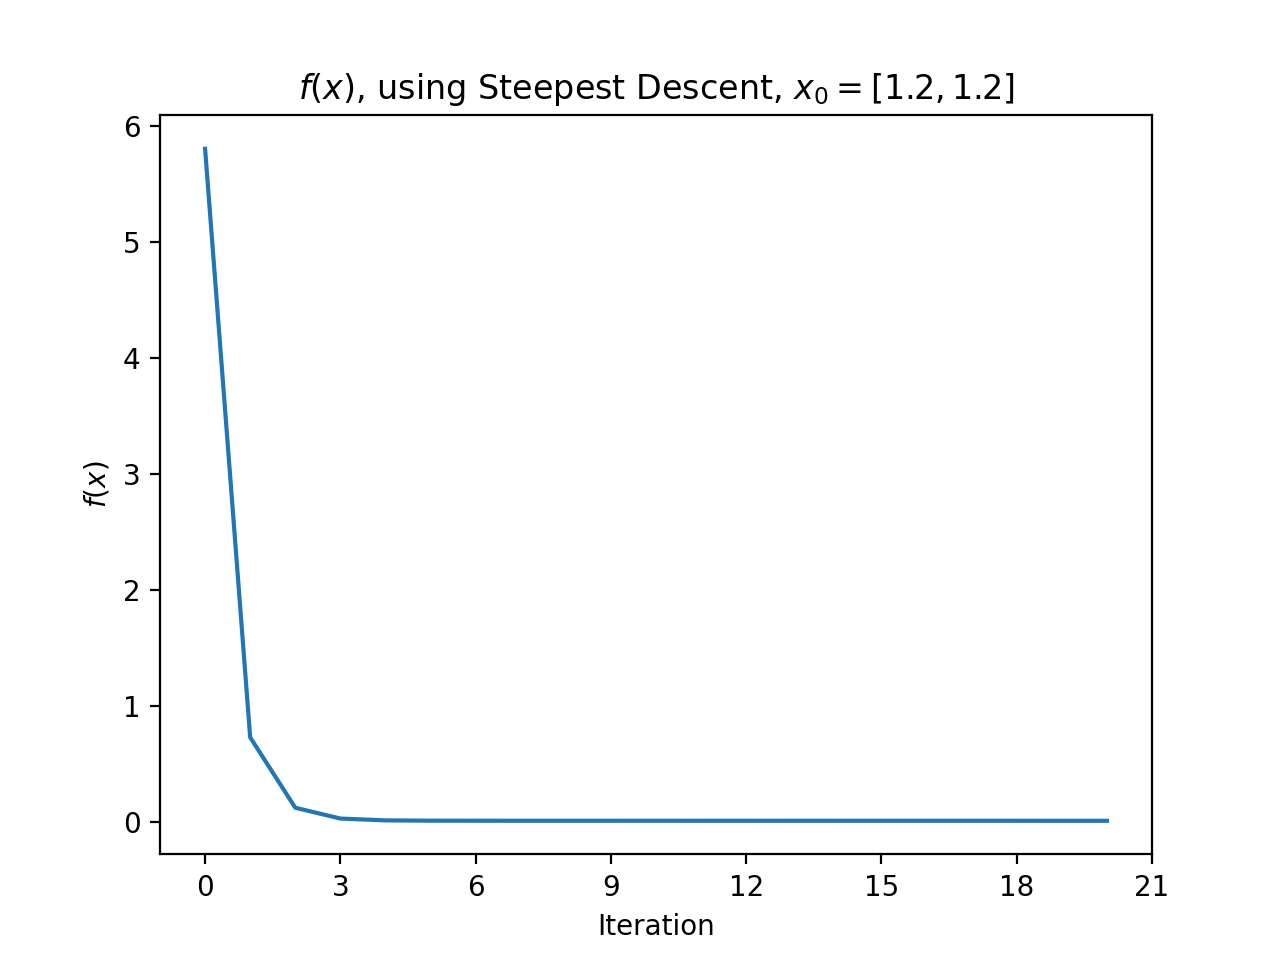
\includegraphics[width=\textwidth]{images/steepest_descent_fx_a.png}
        \caption{$f(x)$, using Steepest Descent, $x_0 = [1.2, 1.2]$}
    \end{minipage}
\end{figure}

\begin{figure}[!tbp]
    \centering
    \begin{minipage}[b]{0.4\textwidth}
        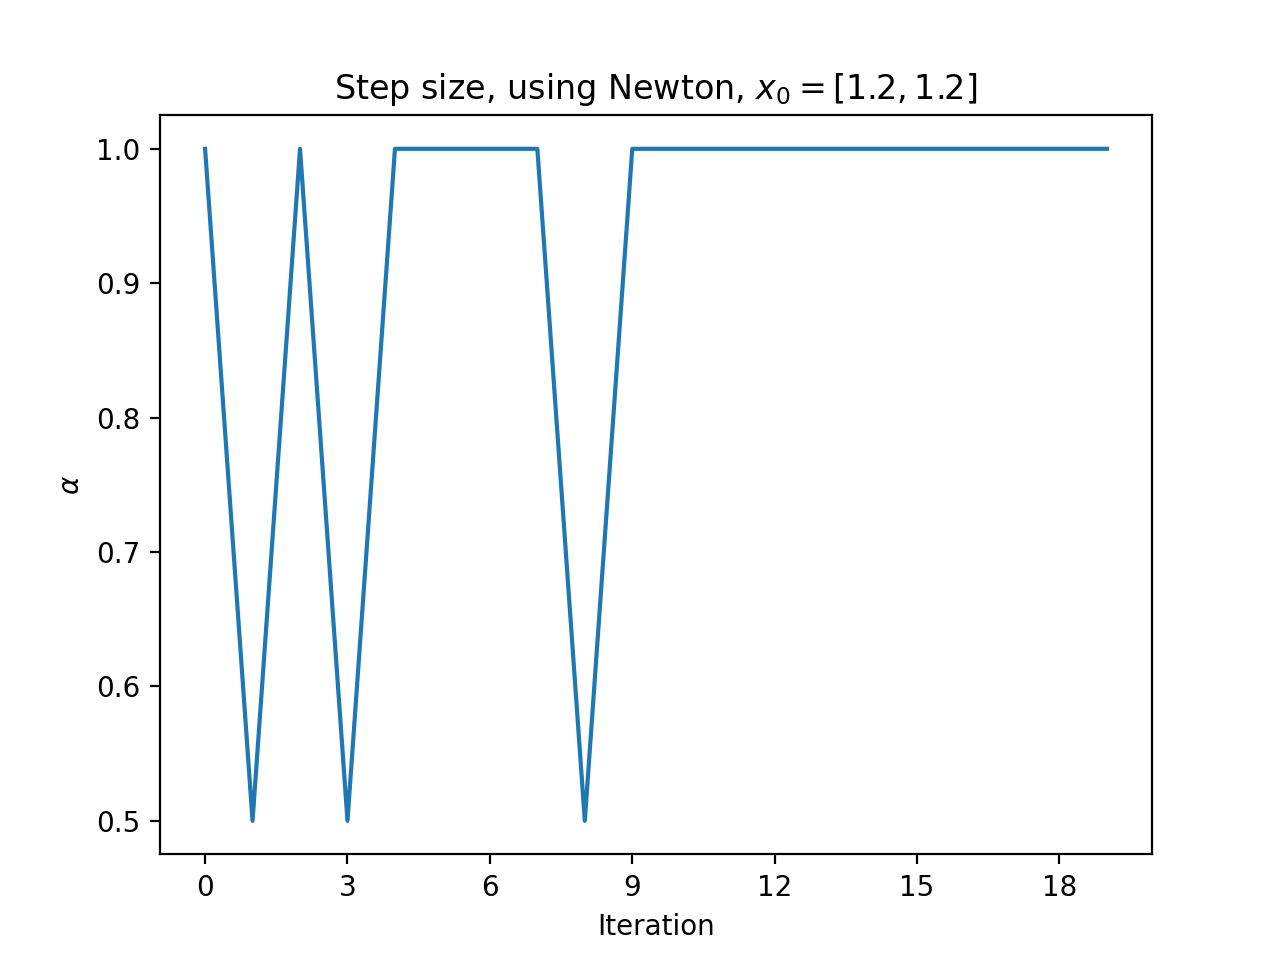
\includegraphics[width=\textwidth]{images/newton_step_size_a.png}
        \caption{Step size, using Newton, $x_0 = [1.2, 1.2]$}
    \end{minipage}
    \hfill
    \begin{minipage}[b]{0.4\textwidth}
        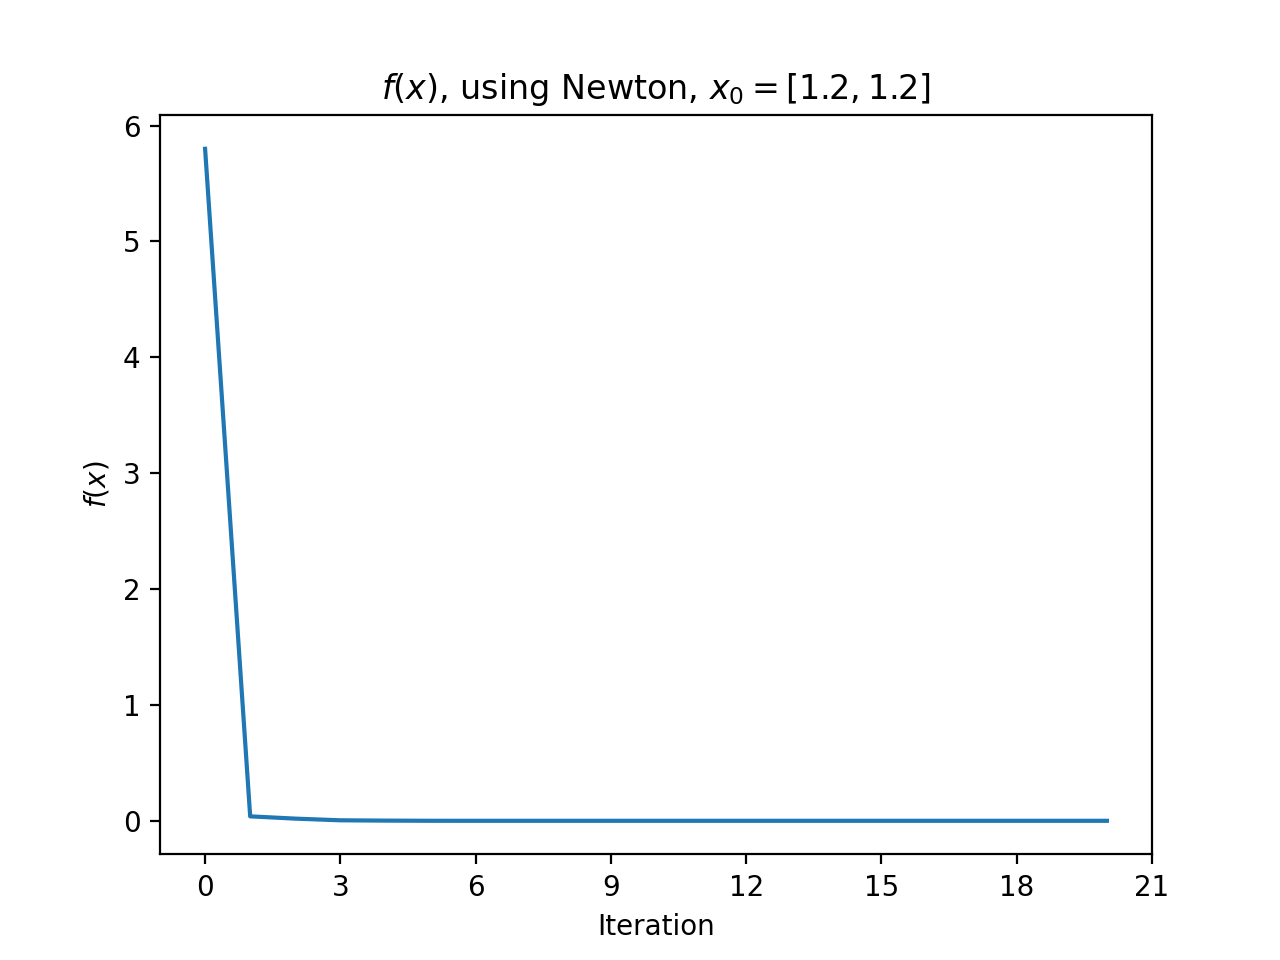
\includegraphics[width=\textwidth]{images/newton_fx_a.png}
        \caption{$f(x)$, using Newton, $x_0 = [1.2, 1.2]$}
    \end{minipage}

\end{figure}

\begin{figure}[!tbp]
    \centering
    \begin{minipage}[b]{0.4\textwidth}
        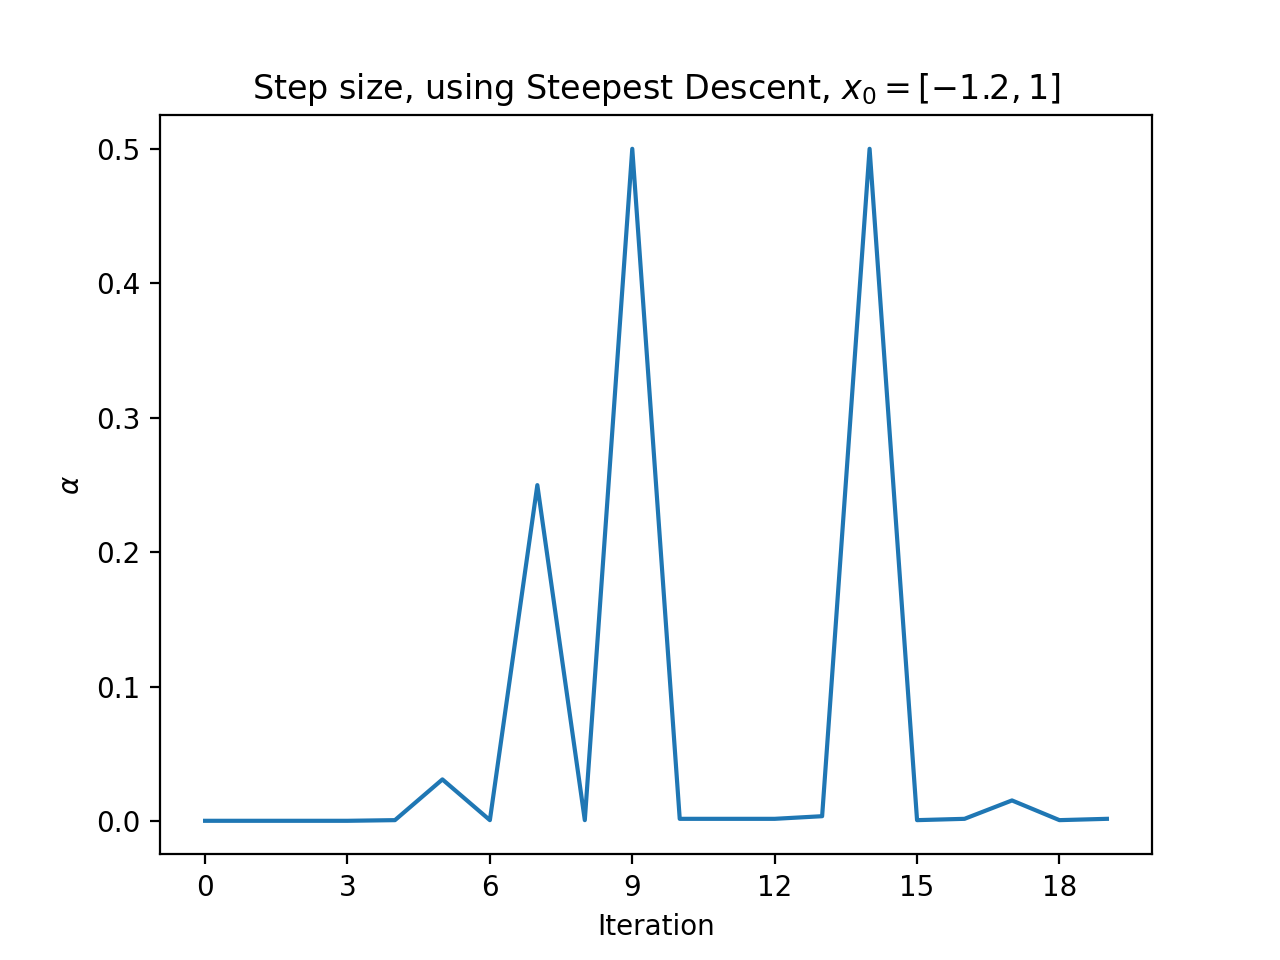
\includegraphics[width=\textwidth]{images/steepest_descent_step_size_b.png}
        \caption{Step size, using Steepest Descent, $x_0 = [-1.2, 1]$}
    \end{minipage}
    \hfill
    \begin{minipage}[b]{0.4\textwidth}
        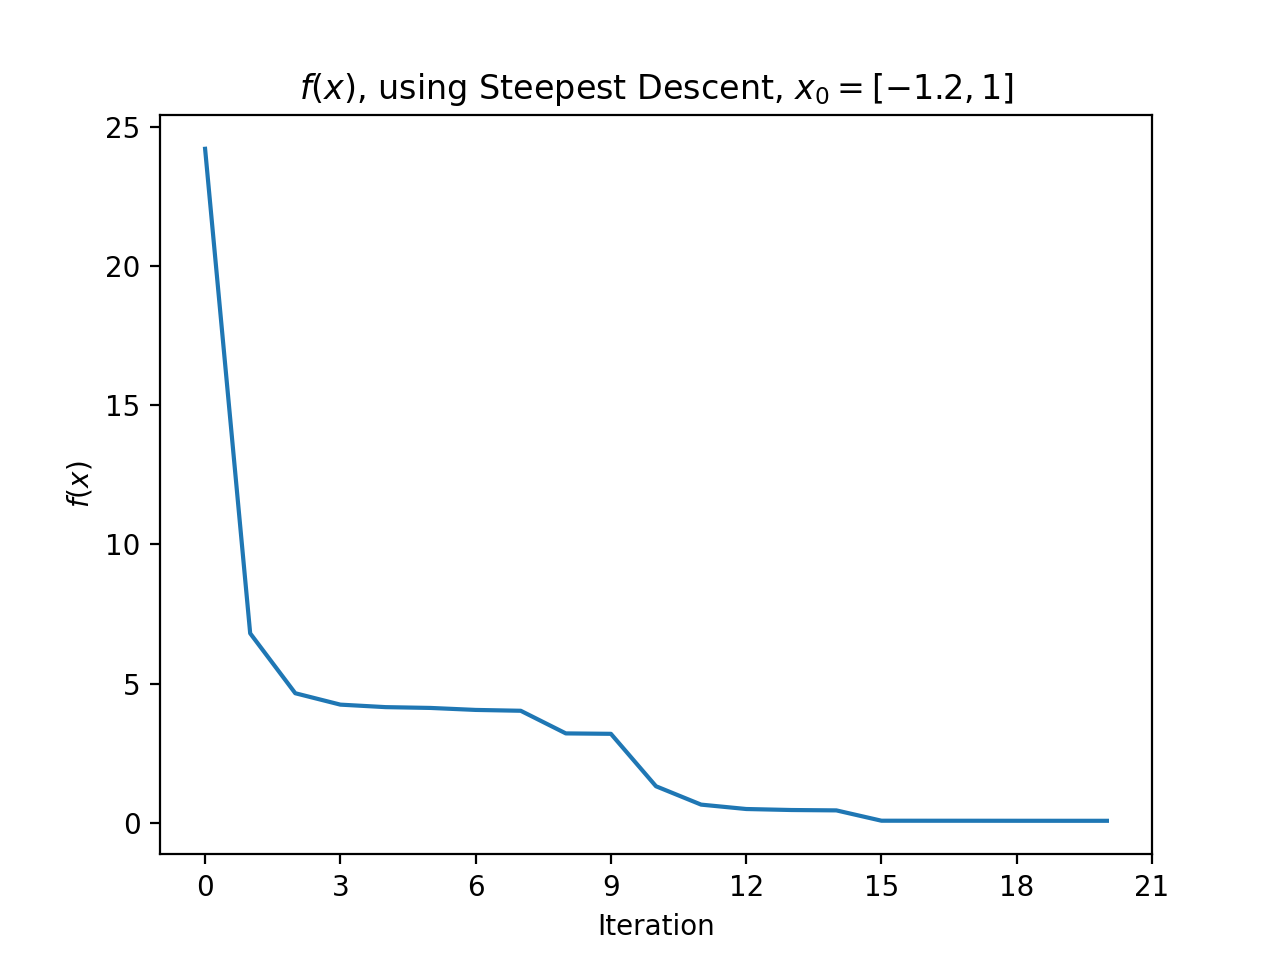
\includegraphics[width=\textwidth]{images/steepest_descent_fx_b.png}
        \caption{$f(x)$, using Steepest Descent, $x_0 = [-1.2, 1]$}
    \end{minipage}
\end{figure}

\begin{figure}[!tbp]
    \centering
    \begin{minipage}[b]{0.4\textwidth}
        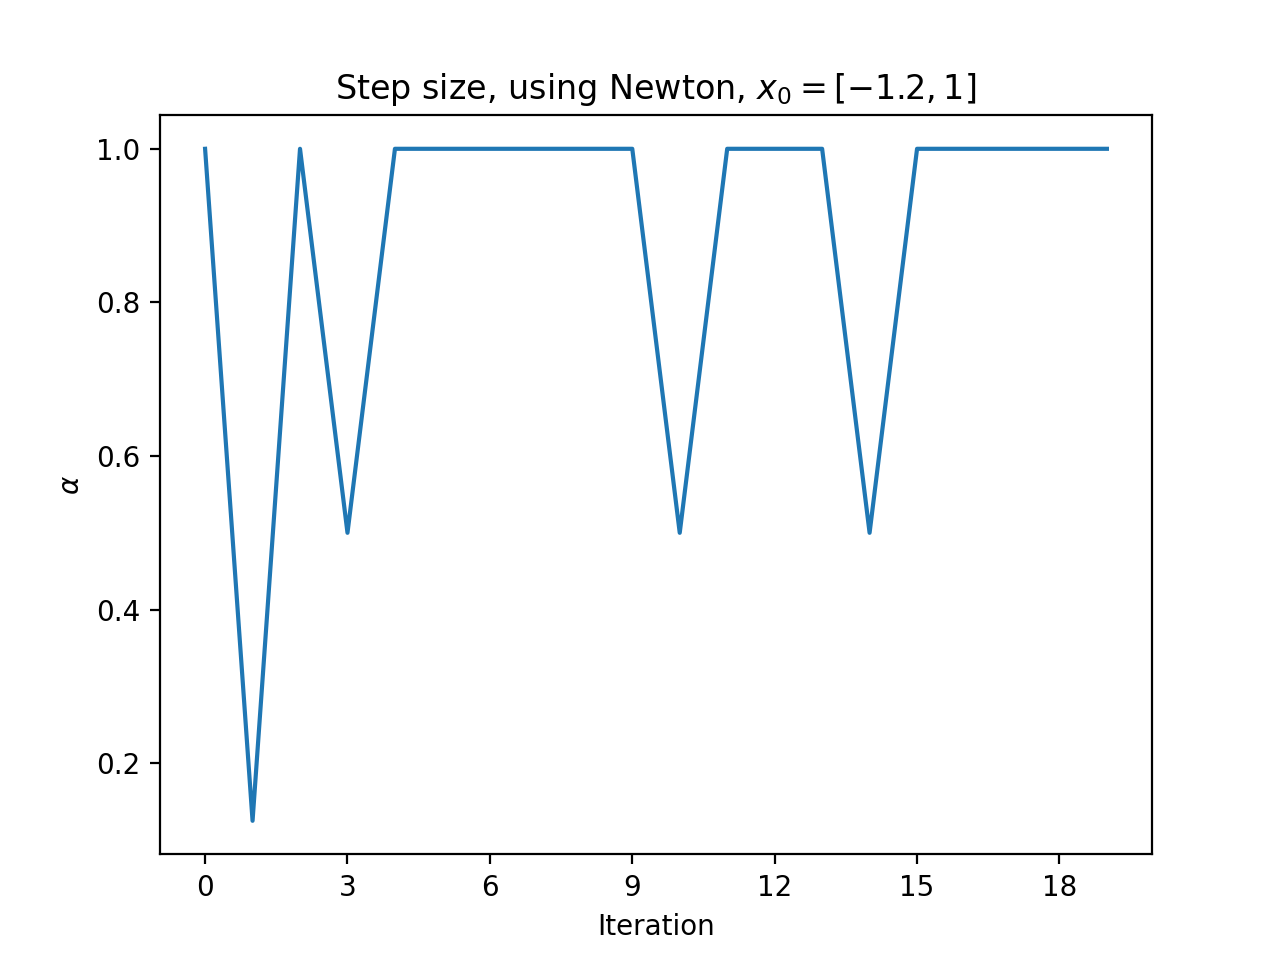
\includegraphics[width=\textwidth]{images/newton_step_size_b.png}
        \caption{Step size, using Newton, $x_0 = [-1.2, 1]$}
    \end{minipage}
    \hfill
    \begin{minipage}[b]{0.4\textwidth}
        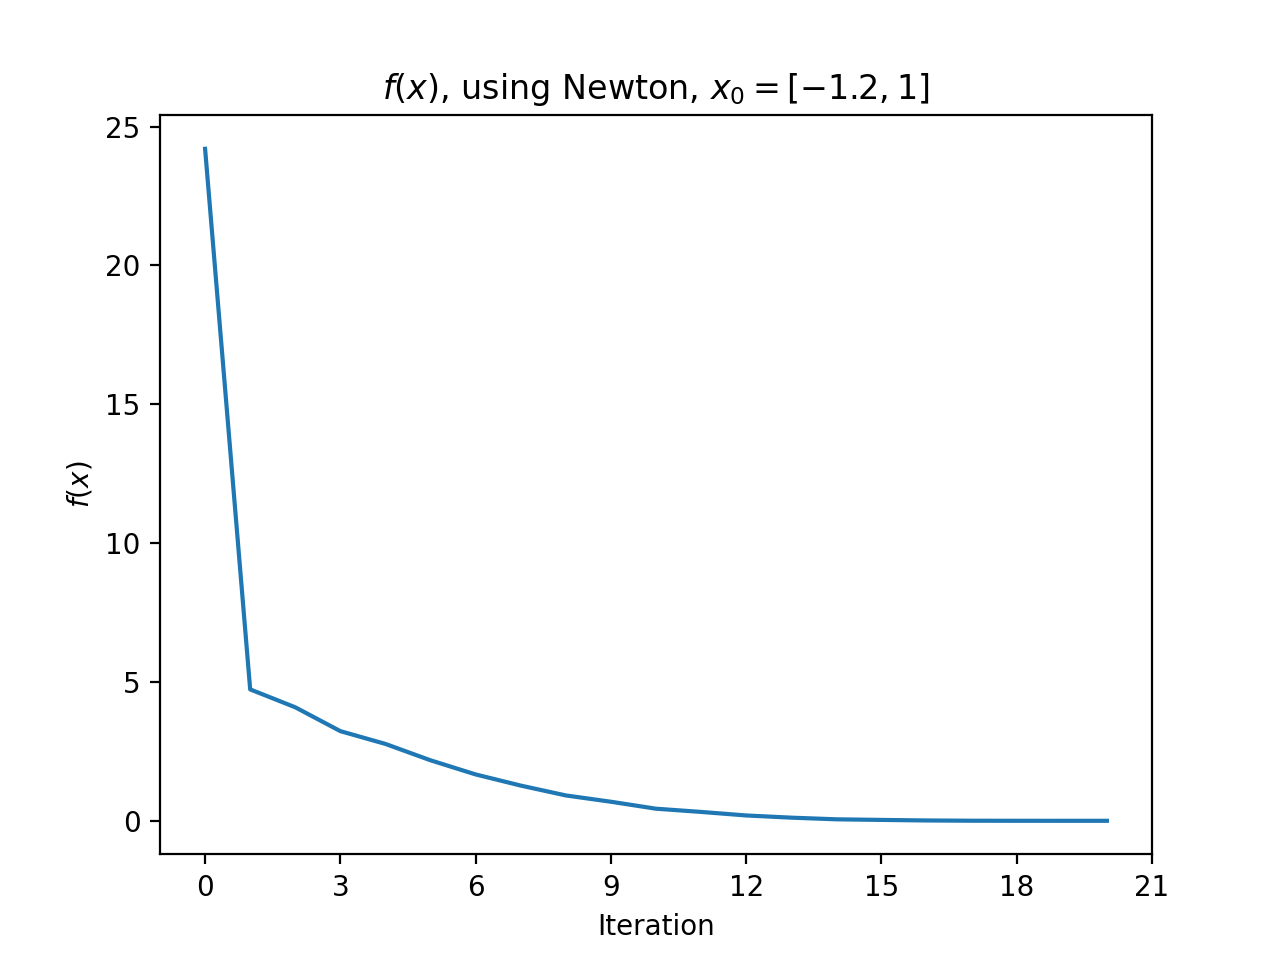
\includegraphics[width=\textwidth]{images/newton_fx_b.png}
        \caption{$f(x)$, using Newton, $x_0 = [-1.2, 1]$}
    \end{minipage}
\end{figure}


\hfill \break %SPACE

\setcounter{section}{4}

\section{Consider the function 
$f(x) = \langle c, x \rangle + \displaystyle\sum_{j=1}^m \log(1-\langle a_j, x\rangle) - \displaystyle\sum_{i=1}^n \log(1-x_i^2)$.
Take $n=5000$ and $m=2000$, and vectors $c$, $a_j$ chosen arbitrarily in 
such a way that $\| a_j \| = 1$. For each of the methods, start the iteration at $x=0$ and stop the iteration when $\| \nabla f(x) \| < \varepsilon$.
Graph $\log(f(x_k) - f(x^*))$ in each iteration, (estimate $f(x^*)$) as best as you can and compare the time of execution of the methods.}


In all the problems it was chosen $c_i=1$ for all $i$. In non of the problems it was possible to use $\varepsilon = 10^{-6}$, since the gradient of the function was always greater than this value, possible due to accumulation of errors. Six iterations 
of each method were used.

The vectors $a_j$ were generated using the following code:

\begin{lstlisting}[language=Python]
import sympy as sp
import sympy.stats as stats

Z = stats.Normal('Z', 0, 1)

n = 5000
m = 2000
A = []

for i in range(m):
    Aj = sp.Matrix(stats.sample(Z, size=n, seed=3527+i))
    norm_Aj = sp.sqrt(sum([a**2 for a in Aj]))
    Aj = (1 / norm_Aj) * Aj # Normalize Aj
    A.append(Aj)
    if i % 100 == 0:
        print(f'{i} vectors generated')

# Save A to a file, where each row is a vector Aj
with open('A.txt', 'w') as f:
    for Aj in A:
        f.write(','.join([str(a) for a in Aj]) + '\n')
\end{lstlisting}

\begin{enumerate}[label=(\alph*)]
    \item Use the gradient method with a fixed step length step, indicating the value of step used and why you chose it.
\end{enumerate}

\paragraph{Solution:}

In this case we used $\alpha = 0.2$ as the step size, since it is a small value that allowed the problem to work without getting out of the domain of the logarithm function. The execution time
of this method was $1.1878$ hours. 

The code used to solve this problem is given by:

\begin{lstlisting}[language=Python]
    import matplotlib.pyplot as plt
    import os
    from time import perf_counter
    from numpy import float16, dot, ones, zeros, log
    from numpy.linalg import norm, solve
    import pandas as pd
    from progress.bar import Bar
    
    n = 5000
    m = 2000
    epsilon = float16(1e-6)
    max_iterations = 6 # Maximum number of iterations
    max_sub_iterations = 3 # Maximum number of sub-iterations
    # C is the vector of ones
    ONE = float16(1)
    TWO = float16(2)
    
    dots = {}
    def optimized_dot(x,y):
        stringxy = str(x) + str(y)
        if stringxy in dots:
            return dots[stringxy]
        result = dot(x,y)
        dots[stringxy] = result
        return result
    
    fs = {}
    def f(x, A):
        stringx = str(x)
        if stringx in fs:
            return fs[stringx]
    
        result = sum(x)
        for j in range(m):
            result -= log(ONE - optimized_dot(A[j],x))
        for i in range(n):
            result -= log(ONE - x[i]*x[i])
    
        fs[stringx] = result
        return result
    
    gradients = {}
    def gradient(x, A):
        stringx = str(x)
        if stringx in gradients:
            return gradients[stringx]
    
        result = ones(n, dtype=float16)
        with Bar('Gradient', fill='#', suffix='%(percent).1f%% - %(eta)ds', max=n) as bar:
            for i in range(n):
                for j in range(m):
                    result[i] += A[j][i] / (ONE - optimized_dot(A[j],x))
                result[i] += TWO * x[i] / (ONE - x[i]*x[i])
                bar.next()
    
        gradients[stringx] = result
        return result
    
    hessians = {}
    def hessian(x, A):
        # We assume its symmetric
        stringx = str(x)
        if stringx in hessians:
            return hessians[stringx]
    
        result = zeros((n,n), dtype=float16)
        with Bar('Hessian', fill='#', suffix='%(percent).1f%% - %(eta)ds', max=n*(n+1)/2) as bar:
            for i in range(n):
                for l in range(i,n):
                    for j in range(m):
                        result[i][l] += A[j][i] * A[j][l] / ((ONE - optimized_dot(A[j],x)) * (ONE - optimized_dot(A[j],x)))
                    if i == l:
                        result[i][l] += TWO* (ONE + x[i]*x[i]) / ((ONE - x[i]*x[i]) * (ONE - x[i]*x[i]))
    
                    result[l][i] = result[i][l]
                    bar.next()
    
        hessians[stringx] = result
        return result
    
    
    def graph(x, y, title, x_label, y_label, filename):
        fig = plt.figure()
        plt.plot(x, y)
        plt.title(title)
        plt.xlabel(x_label)
        plt.gca().xaxis.set_major_locator(plt.MaxNLocator(integer=True))
        plt.ylabel(y_label)
        filename = "images" + os.sep + filename + ".png"
        fig.savefig(filename, dpi=fig.dpi)
        plt.clf()
    
    
    A = []
    df = pd.read_csv('A.txt', header=None)
    data = df.values
    for j in range(m):
        # Save data[j] as numpy array of float16
        A.append(data[j].astype(float16))
    print("A loaded")
    
    time0 = perf_counter() 
    
    ## Gradient method with constant step size alpha
    
    alpha = float16(0.2) # Small constant alpha
    X = [zeros(n, dtype=float16)]
    Fx = [f(X[-1],A)]
    P = [- gradient(X[-1], A)]
    gradient_norms = [norm(P[-1])]
    
    iterations = 0
    while (gradient_norms[-1] > epsilon) and (iterations < max_iterations):
        print("Iteration", iterations)
        print("Norm of gradient:", gradient_norms[-1])
        print("f(x_k):", Fx[-1])
        print("x_k:", X[-1]) 
        iterations += 1
        X.append(X[-1] + alpha * P[-1]) # X_k+1 = X_k + alpha * P_k
        Fx.append(f(X[-1], A))
        P.append(- gradient(X[-1], A))
        gradient_norms.append(norm(P[-1]))
    
        
    
    # End timer
    time1 = perf_counter()
    
    print("Gradient method with constant step size alpha =", alpha, "completed")
    print("Iterations:", iterations)
    print("Total time elapsed:", (time1 - time0)/3600, "hours")
    
    graph(range(iterations+1), Fx, "f(x) vs iterations", "Iteration", "f(x)", "5ai")
    graph(range(iterations+1), gradient_norms, "Norm of gradient vs iterations", "Iteration", "Norm of gradient", "5aii")
    
\end{lstlisting}

\begin{enumerate}[label=(\alph*)]
    \setcounter{enumi}{1}
    \item Use the gradient method with \textit{backtracking}.
\end{enumerate}

\paragraph{Solution:}

Here we used the backtracking method with a initial alpha of $0.25$, $\rho = 0.5$ and $c = 0.5$. The execution time of this method was $1.0337$ hours.
The code used to solve this problem is given by:

\begin{lstlisting}[language=Python]
alpha = float16(0.25) # Initial alpha
rho = float16(0.5)
c = float16(0.5)
X = [zeros(n, dtype=float16)]
Fx = [f(X[-1],A)]
ALPHAS = [alpha]
P = [- gradient(X[-1], A)]
gradient_norms = [norm(P[-1])]
iterations = 0

while (gradient_norms[-1] > epsilon) and (iterations < max_iterations):
    print("Iteration", iterations)
    print("Norm of gradient:", gradient_norms[-1])
    print("f(x_k):", Fx[-1])
    print("x_k:", X[-1]) 
    print("Alpha:", ALPHAS[-1])

    iterations += 1
    sub_iterations = 0

    while f(X[-1] + ALPHAS[-1] * P[-1], A) > f(X[-1], A) + c * ALPHAS[-1] * optimized_dot(gradient(X[-1], A), P[-1]) and sub_iterations < max_sub_iterations:
        sub_iterations += 1
        ALPHAS[-1] = rho * ALPHAS[-1]
    
    X.append(X[-1] + ALPHAS[-1] * P[-1]) # X_k+1 = X_k + alpha * P_k
    Fx.append(f(X[-1], A))
    P.append(- gradient(X[-1], A))
    gradient_norms.append(norm(P[-1]))
    ALPHAS.append(alpha)

# End timer
time2 = perf_counter()

print("Gradient method with backtraking completed")
print("Iterations:", iterations)
print("Total time elapsed:", (time2 - time1)/3600, "hours")

graph(range(iterations+1), Fx, "f(x) vs iterations", "Iteration", "f(x)", "5bi")
graph(range(iterations+1), gradient_norms, "Norm of gradient vs iterations", "Iteration", "Norm of gradient", "5bii")
graph(range(iterations+1), ALPHAS, "Alpha vs iterations", "Iteration", "Alpha", "5biii")

\end{lstlisting}

\begin{enumerate}[label=(\alph*)]
    \setcounter{enumi}{2}
    \item Use the gradient method with \textit{backtracking} and Goldstein or Wolfe conditions.
\end{enumerate}


\paragraph{Solution:}

The initial alpha was set to $0.25$, $c_1 = 10^{-4}$ and $c_2 = 0.9$. And we used the Wolfe conditions. The execution time of this method was $0.6928$ hours.
The code used to solve this problem is given by:

\begin{lstlisting}[language=Python]
    alpha = float16(0.25) # Initial alpha
    c_1 = float16(10e-4)
    c_2 = float16(0.9)
    X = [zeros(n, dtype=float16)]
    Fx = [f(X[-1],A)]
    ALPHAS = [alpha]
    P = [- gradient(X[-1], A)]
    gradient_norms = [norm(P[-1])]
    iterations = 0
    
    while (gradient_norms[-1] > epsilon) and (iterations < max_iterations):
        print("Iteration", iterations)
        print("Norm of gradient:", gradient_norms[-1])
        print("f(x_k):", Fx[-1])
        print("x_k:", X[-1]) 
        print("Alpha:", ALPHAS[-1])
    
        iterations += 1
        sub_iterations = 0
    
        while (f(X[-1] + ALPHAS[-1] * P[-1], A) > f(X[-1], A) + c_1 * ALPHAS[-1] * optimized_dot(gradient(X[-1], A), P[-1]) or (- optimized_dot(gradient(X[-1] + ALPHAS[-1] * P[-1], A), P[-1]) > - c_2 * optimized_dot(gradient(X[-1], A), P[-1]))) and sub_iterations < max_sub_iterations:
            sub_iterations += 1
            ALPHAS[-1] = rho * ALPHAS[-1]
        
        X.append(X[-1] + ALPHAS[-1] * P[-1]) # X_k+1 = X_k + alpha * P_k
        Fx.append(f(X[-1], A))
        P.append(- gradient(X[-1], A))
        gradient_norms.append(norm(P[-1]))
        ALPHAS.append(alpha)
    
    # End timer
    time3 = perf_counter()
    
    print("Gradient method with backtraking and Wolfe conditions completed")
    print("Iterations:", iterations)
    print("Total time elapsed:", (time3 - time2)/3600, "hours")
    
    graph(range(iterations+1), Fx, "f(x) vs iterations", "Iteration", "f(x)", "5ci")
    graph(range(iterations+1), gradient_norms, "Norm of gradient vs iterations", "Iteration", "Norm of gradient", "5cii")
    graph(range(iterations+1), ALPHAS, "Alpha vs iterations", "Iteration", "Alpha", "5ciii")
\end{lstlisting}

\begin{enumerate}[label=(\alph*)]
    \setcounter{enumi}{3}
    \item Use the Newton method with a fixed step length step.
\end{enumerate}

\paragraph{Solution:}

We used a step size of $0.2$ for the Newton method. The execution time of this method could not be calculated since 
each iteration takes more than $30$ days, even after multiple optimizations. The code used to solve this problem is given by:

\begin{lstlisting}[language=Python]
alpha = float16(0.2) # Small constant alpha
X = [zeros(n, dtype=float16)]
Fx = [f(X[-1],A)]
P = [solve(hessian(X[-1], A), -gradient(X[-1], A))]
iterations = 0

while iterations < max_iterations:
    print("Iteration", iterations)
    print("f(x_k):", Fx[-1])
    print("x_k:", X[-1]) 
    iterations += 1
    X.append(X[-1] + alpha * P[-1]) # X_k+1 = X_k + alpha * P_k
    Fx.append(f(X[-1], A))
    P.append(solve(hessian(X[-1], A), -gradient(X[-1], A)))

# End timer
time4 = perf_counter()

print("Newton method with constant step size alpha =", alpha, "completed")
print("Iterations:", iterations)
print("Total time elapsed:", (time4 - time3)/3600, "hours")

graph(range(iterations+1), Fx, "f(x) vs iterations", "Iteration", "f(x)", "5di")
\end{lstlisting}



\begin{figure}[!tbp]
    \centering
    \begin{minipage}[b]{0.4\textwidth}
        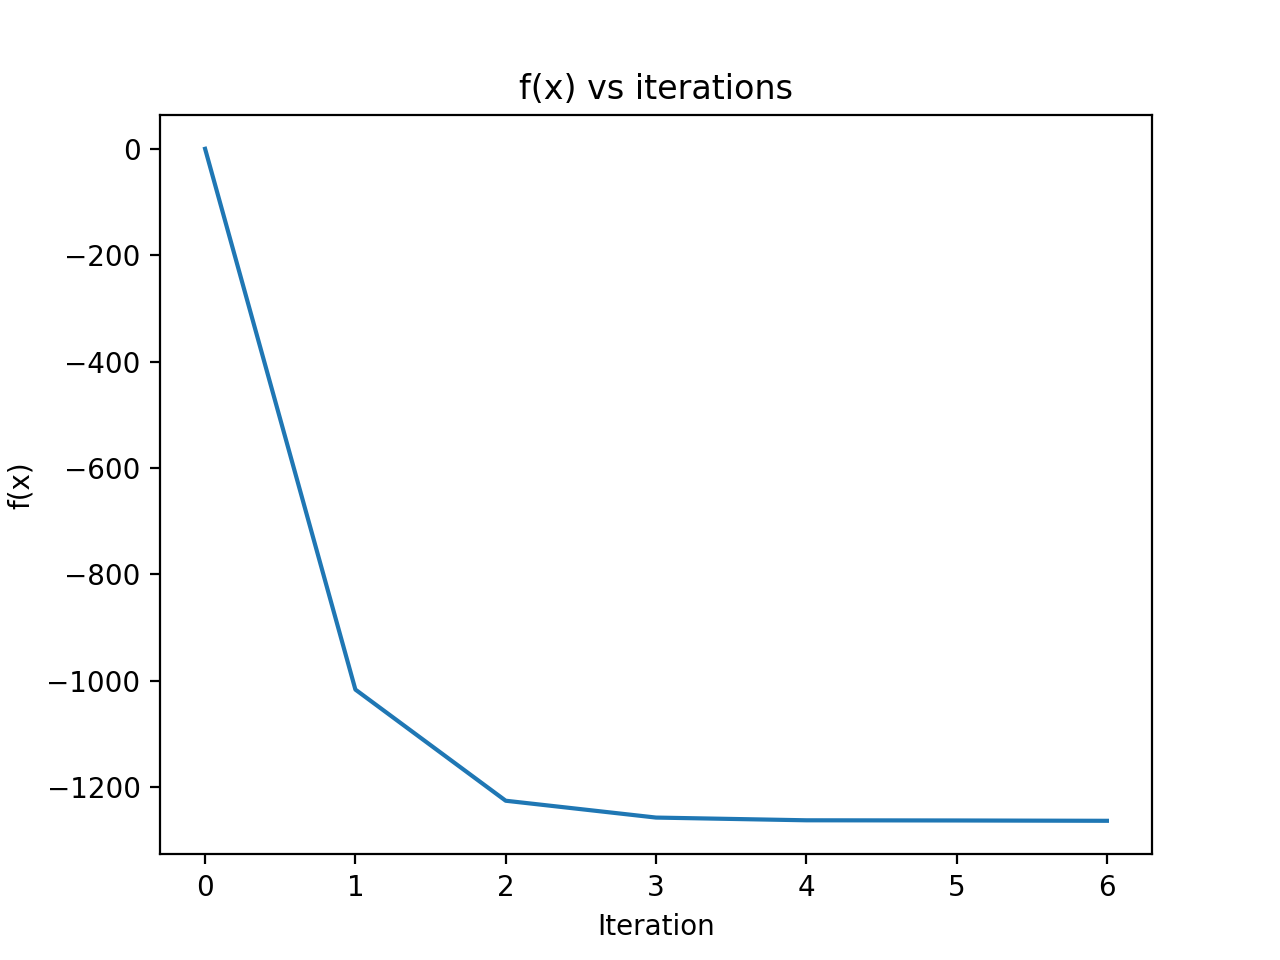
\includegraphics[width=\textwidth]{images/5ai.png}
        \caption{$f(x)$, using gradient method, $x_0 = 0$, $\alpha = 0.2$}
    \end{minipage}
    \hfill
    \begin{minipage}[b]{0.4\textwidth}
        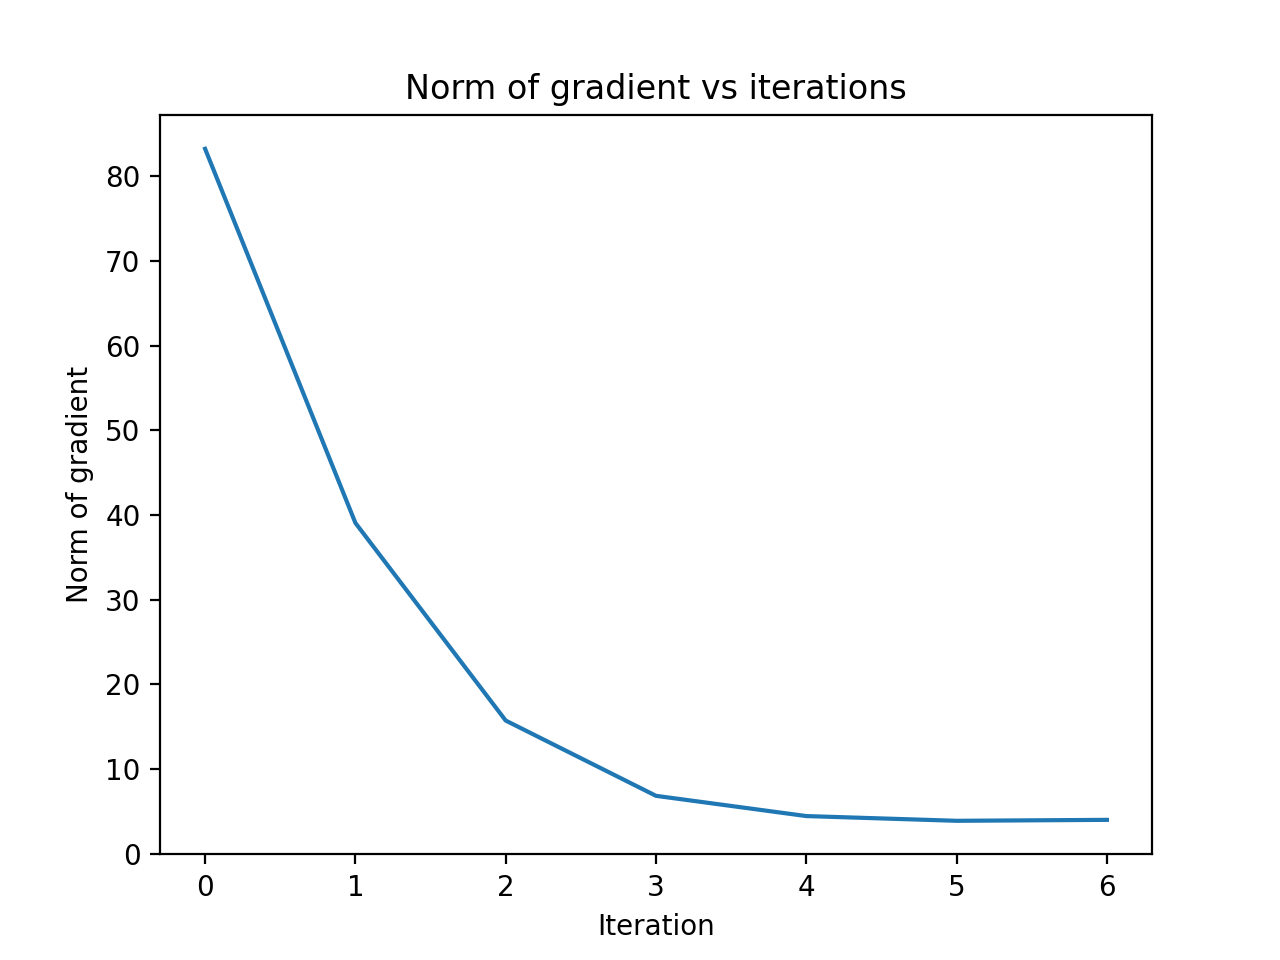
\includegraphics[width=\textwidth]{images/5aii.png}
        \caption{Norm of gradient, using gradient method, $x_0 = 0$, $\alpha = 0.2$}
    \end{minipage}
\end{figure}

\begin{figure}[!tbp]
    \centering
    \begin{minipage}[b]{0.266\textwidth}
        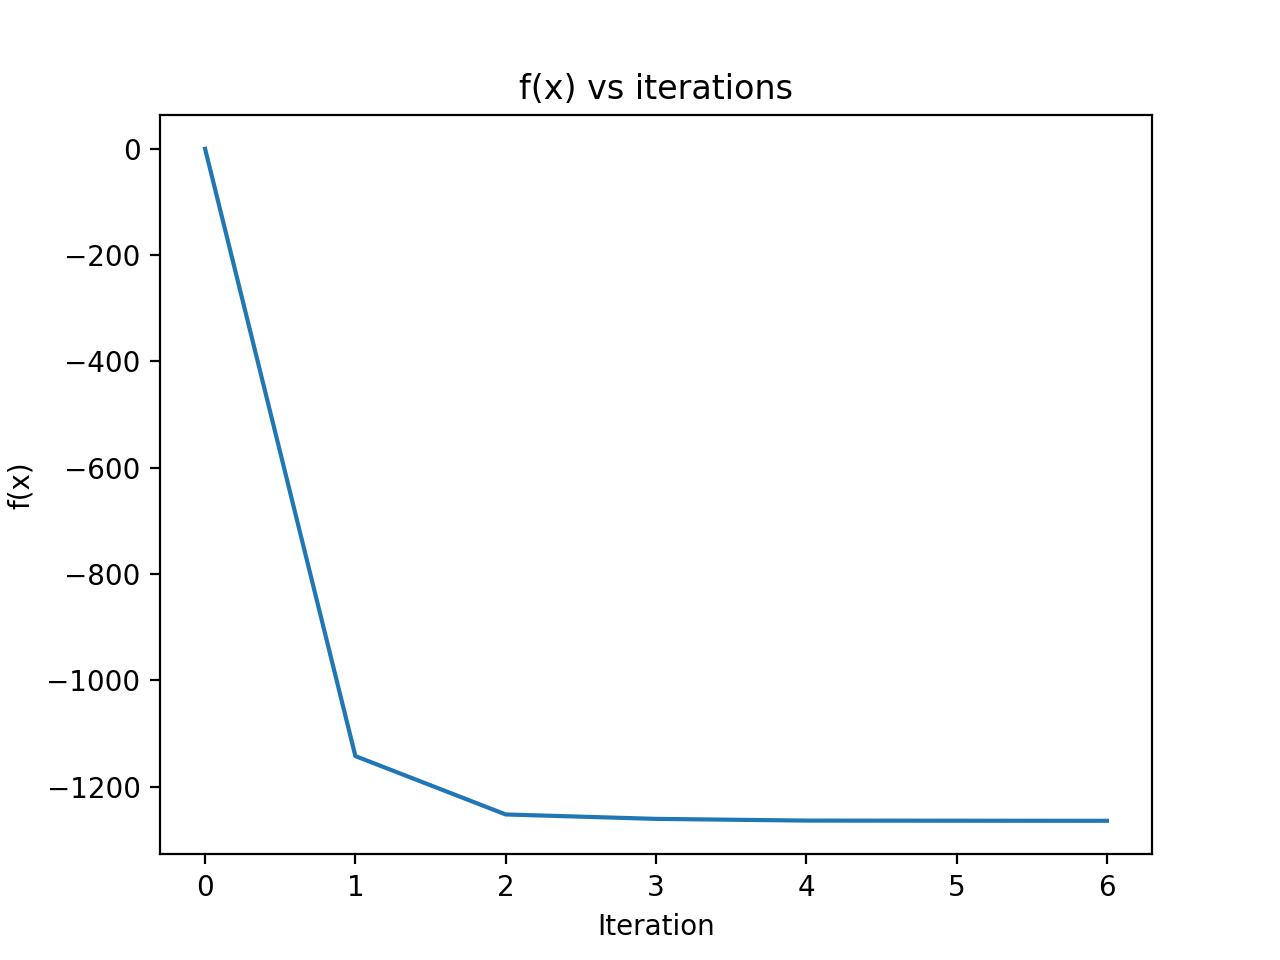
\includegraphics[width=\textwidth]{images/5bi.png}
        \caption{$f(x)$, using gradient method with backtracking, $x_0 = 0$, $\alpha = 0.25$, $\rho = 0.5$, $c = 0.5$}
    \end{minipage}
    \hfill
    \begin{minipage}[b]{0.266\textwidth}
        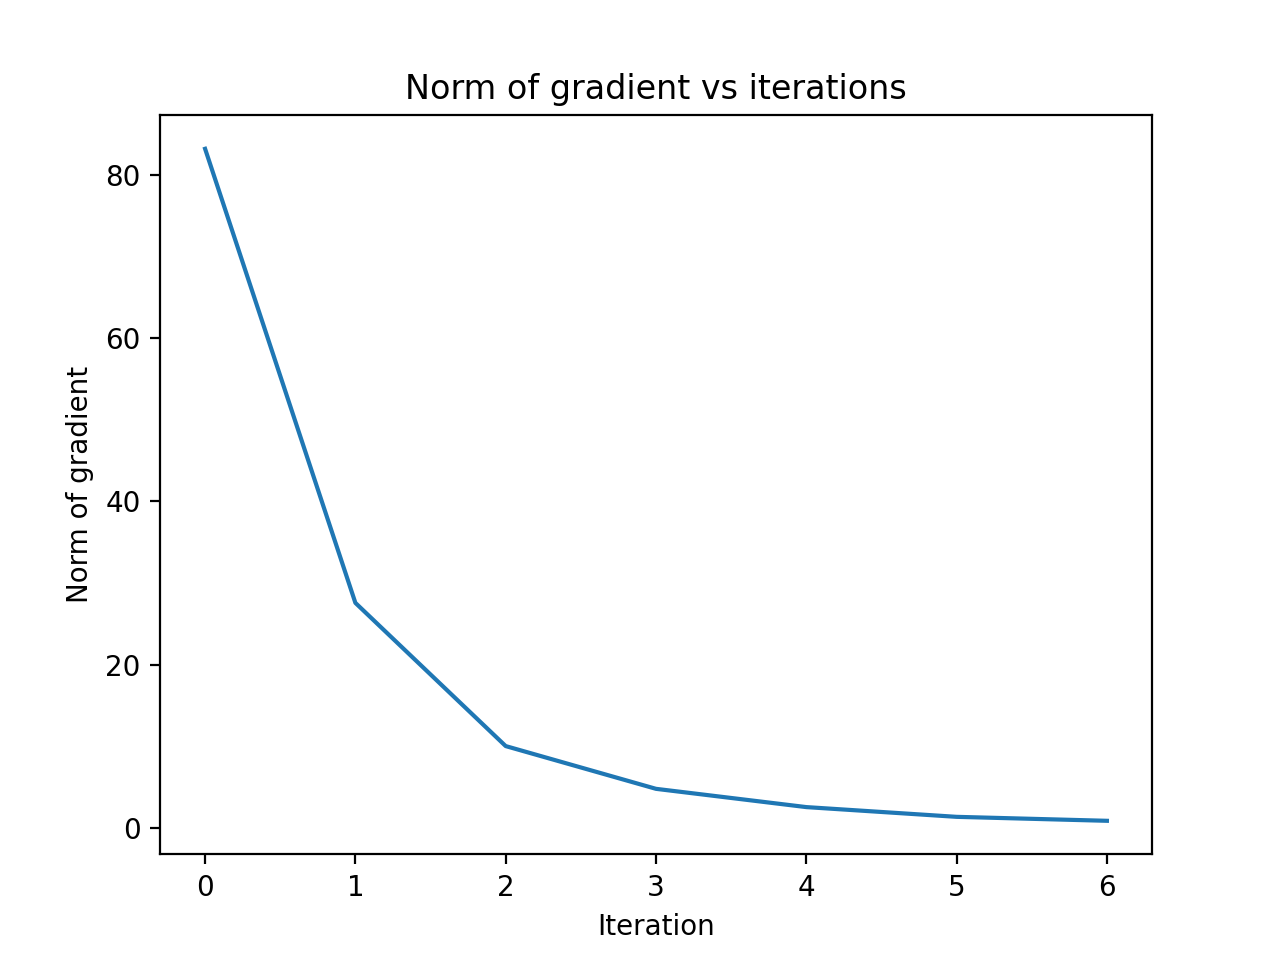
\includegraphics[width=\textwidth]{images/5bii.png}
        \caption{Norm of gradient, using gradient method with backtracking, $x_0 = 0$, $\alpha = 0.25$, $\rho = 0.5$, $c = 0.5$}
    \end{minipage}
    \hfill
    \begin{minipage}[b]{0.266\textwidth}
        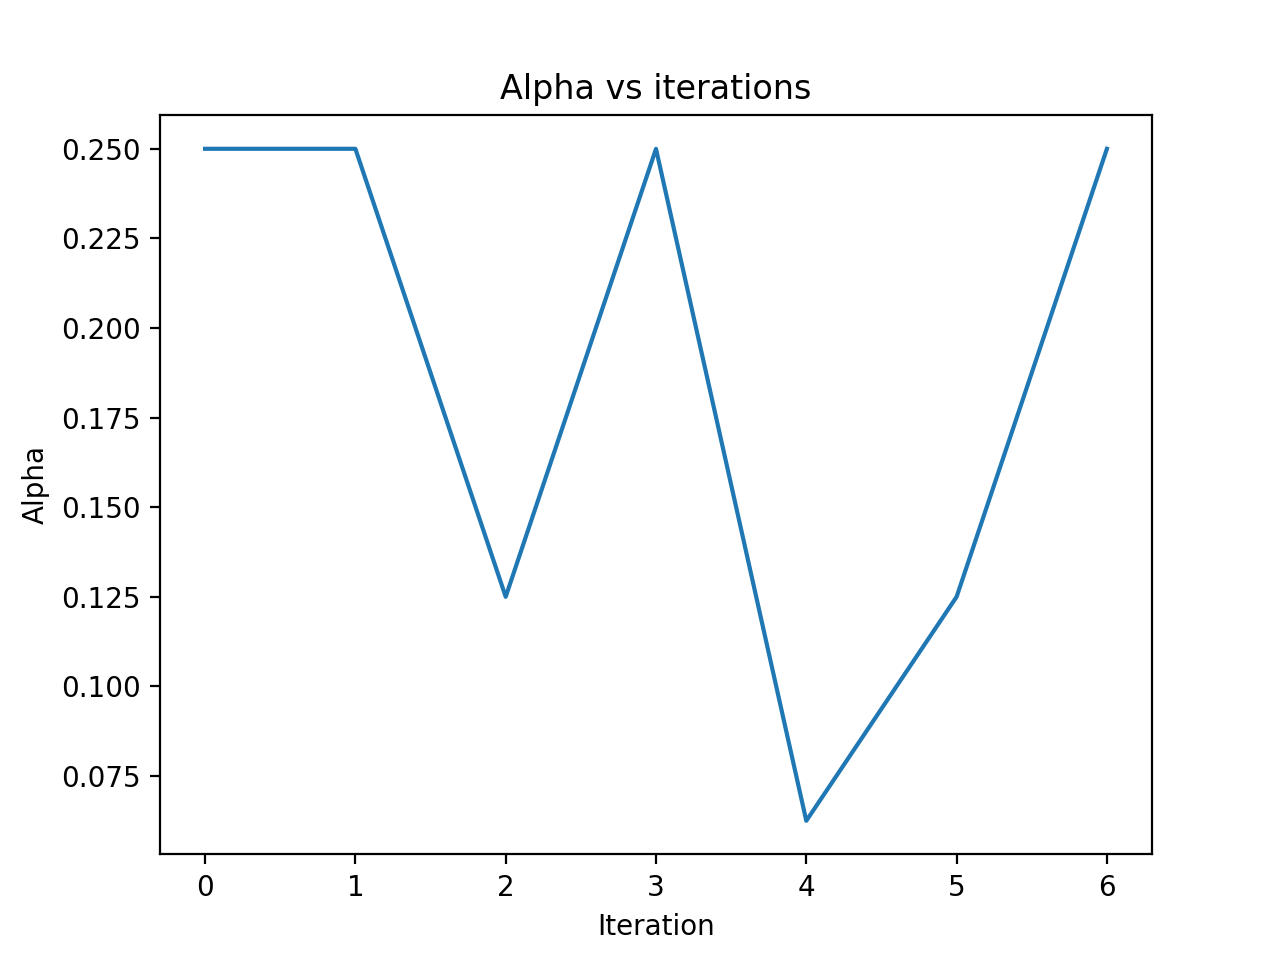
\includegraphics[width=\textwidth]{images/5biii.png}
        \caption{Alpha, using gradient method with backtracking, $x_0 = 0$, $\alpha = 0.25$, $\rho = 0.5$, $c = 0.5$}
    \end{minipage}
\end{figure}

\begin{figure}[!tbp]
    \centering
    \begin{minipage}[b]{0.266\textwidth}
        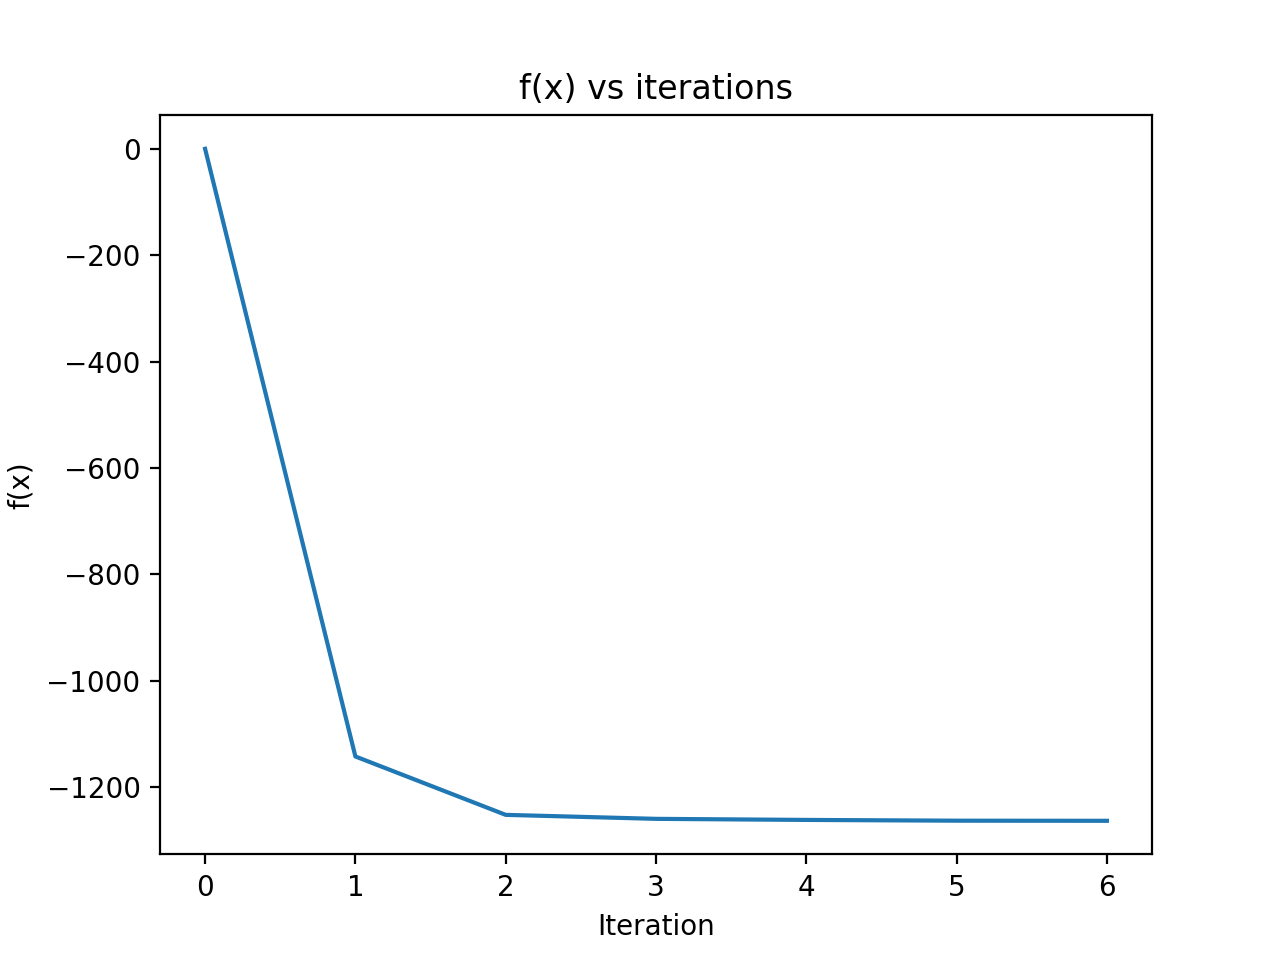
\includegraphics[width=\textwidth]{images/5ci.png}
        \caption{$f(x)$, using gradient method with backtracking and Wolfe conditions, $x_0 = 0$, $\alpha = 0.25$, $c_1 = 10^{-4}$, $c_2 = 0.9$}
    \end{minipage}
    \hfill
    \begin{minipage}[b]{0.266\textwidth}
        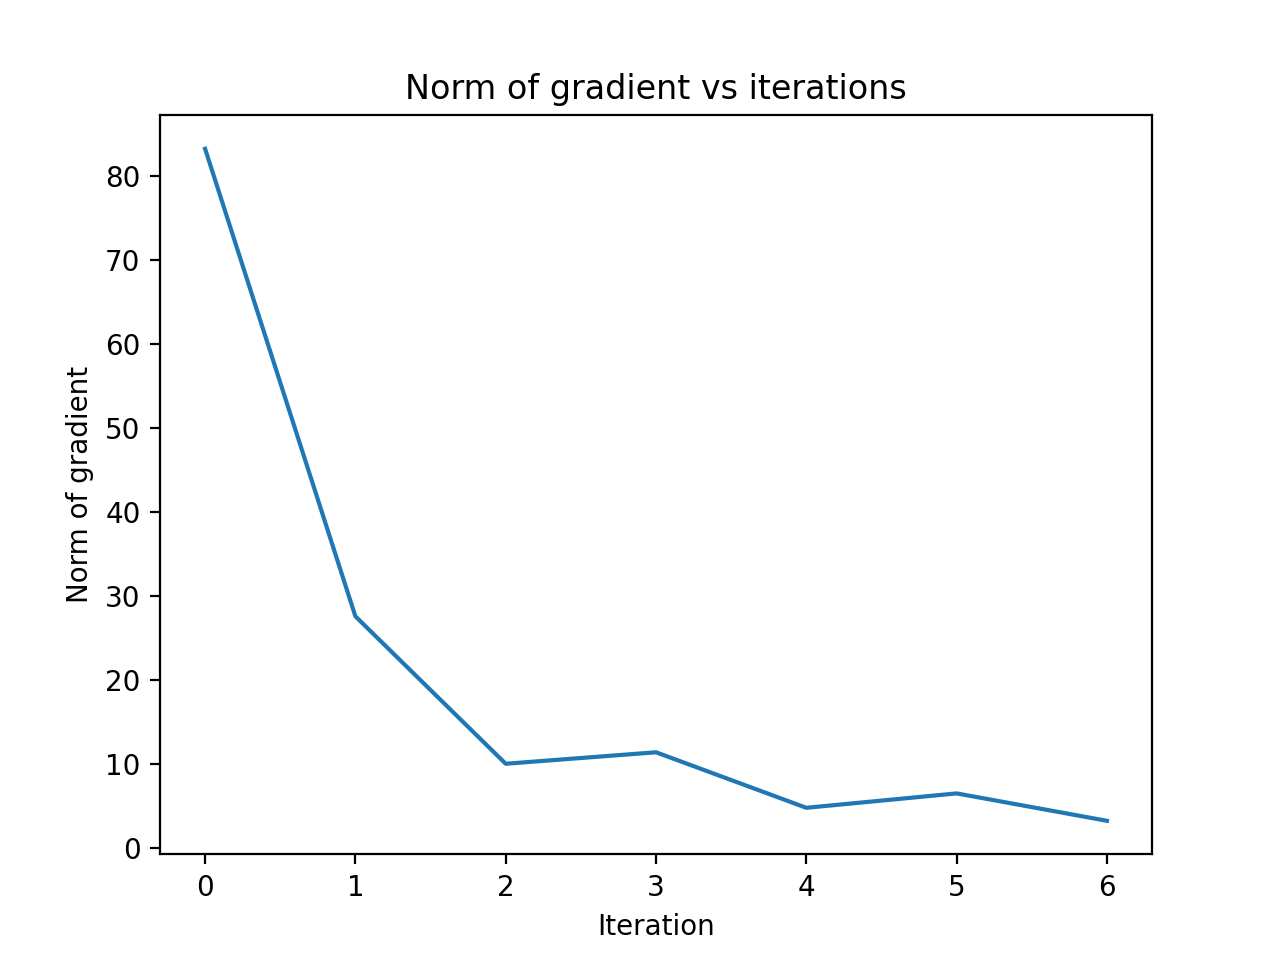
\includegraphics[width=\textwidth]{images/5cii.png}
        \caption{Norm of gradient, using gradient method with backtracking and Wolfe conditions, $x_0 = 0$, $\alpha = 0.25$, $c_1 = 10^{-4}$, $c_2 = 0.9$}
    \end{minipage}
    \hfill
    \begin{minipage}[b]{0.266\textwidth}
        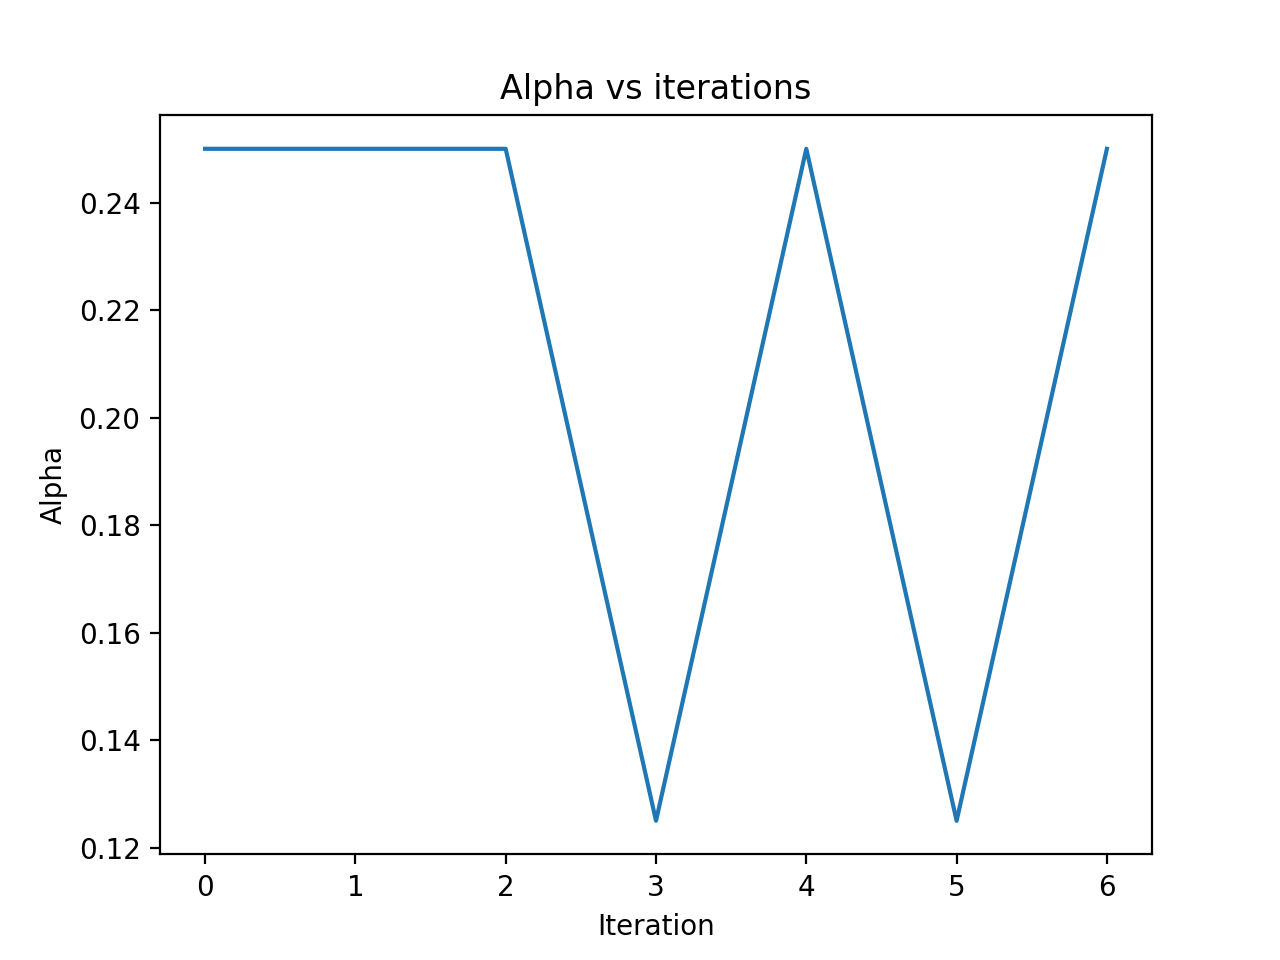
\includegraphics[width=\textwidth]{images/5ciii.png}
        \caption{Alpha, using gradient method with backtracking and Wolfe conditions, $x_0 = 0$, $\alpha = 0.25$, $c_1 = 10^{-4}$, $c_2 = 0.9$}
    \end{minipage}
\end{figure}



\end{document}